\section{Architecting TLBs in DRAM } 
\label{sec:stackedTLB}

\noindent When the application working set exceeds the TLB coverage
provided by UCAT (e.g. $GUPS$), UCAT does not reduce the number of
memory accesses on an LLT miss. Reducing the number of memory accesses
on an LLT miss improves memory access bandwidth and also reduces the
effective LLT miss latency.

To address this problem, we propose to increase TLB coverage and
extend the processor TLB hierarchy by architecting {\em TLBs in DRAM
(DRAM-TLB)}. The DRAM-TLB logically sits between the on-die shared LLT
(or UCAT) and the page tables in memory and is first consulted on an
LLT (or UCAT) miss before walking the page table (see
Figure~\ref{fig:stacked_tlb}).

% \noindent Recent proposals extend the processor cache hierarchy by
% architecting stacked memory as a high capacity hardware-managed DRAM
% cache~\cite{BEAR, moin2012, unison, loh2011, jaewoong2012}. Similarly,

\begin{figure*}[t] 
  \vspace{-0. in} \centering
%  \centerline{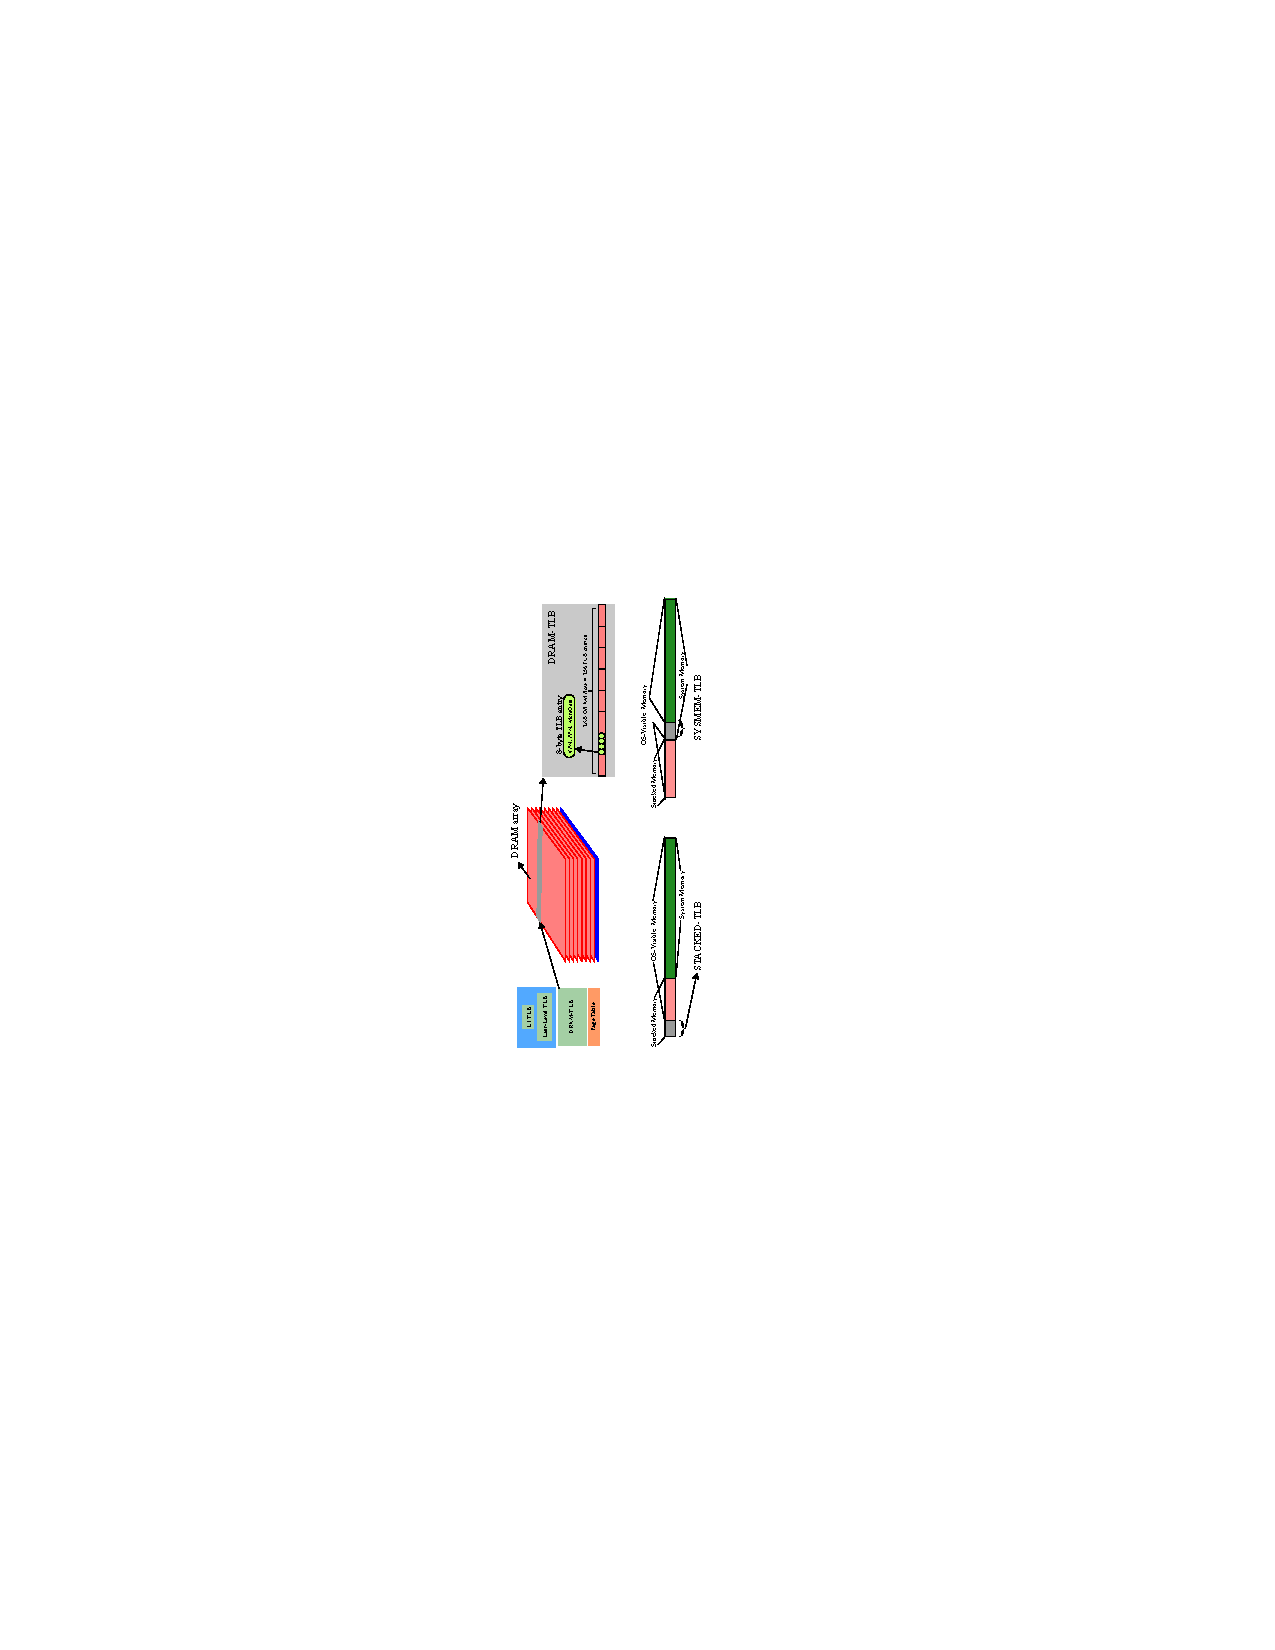
\psfig{file=FIGURES/stacked_tlb,angle=-90,width=\columnwidth}}
   \centerline{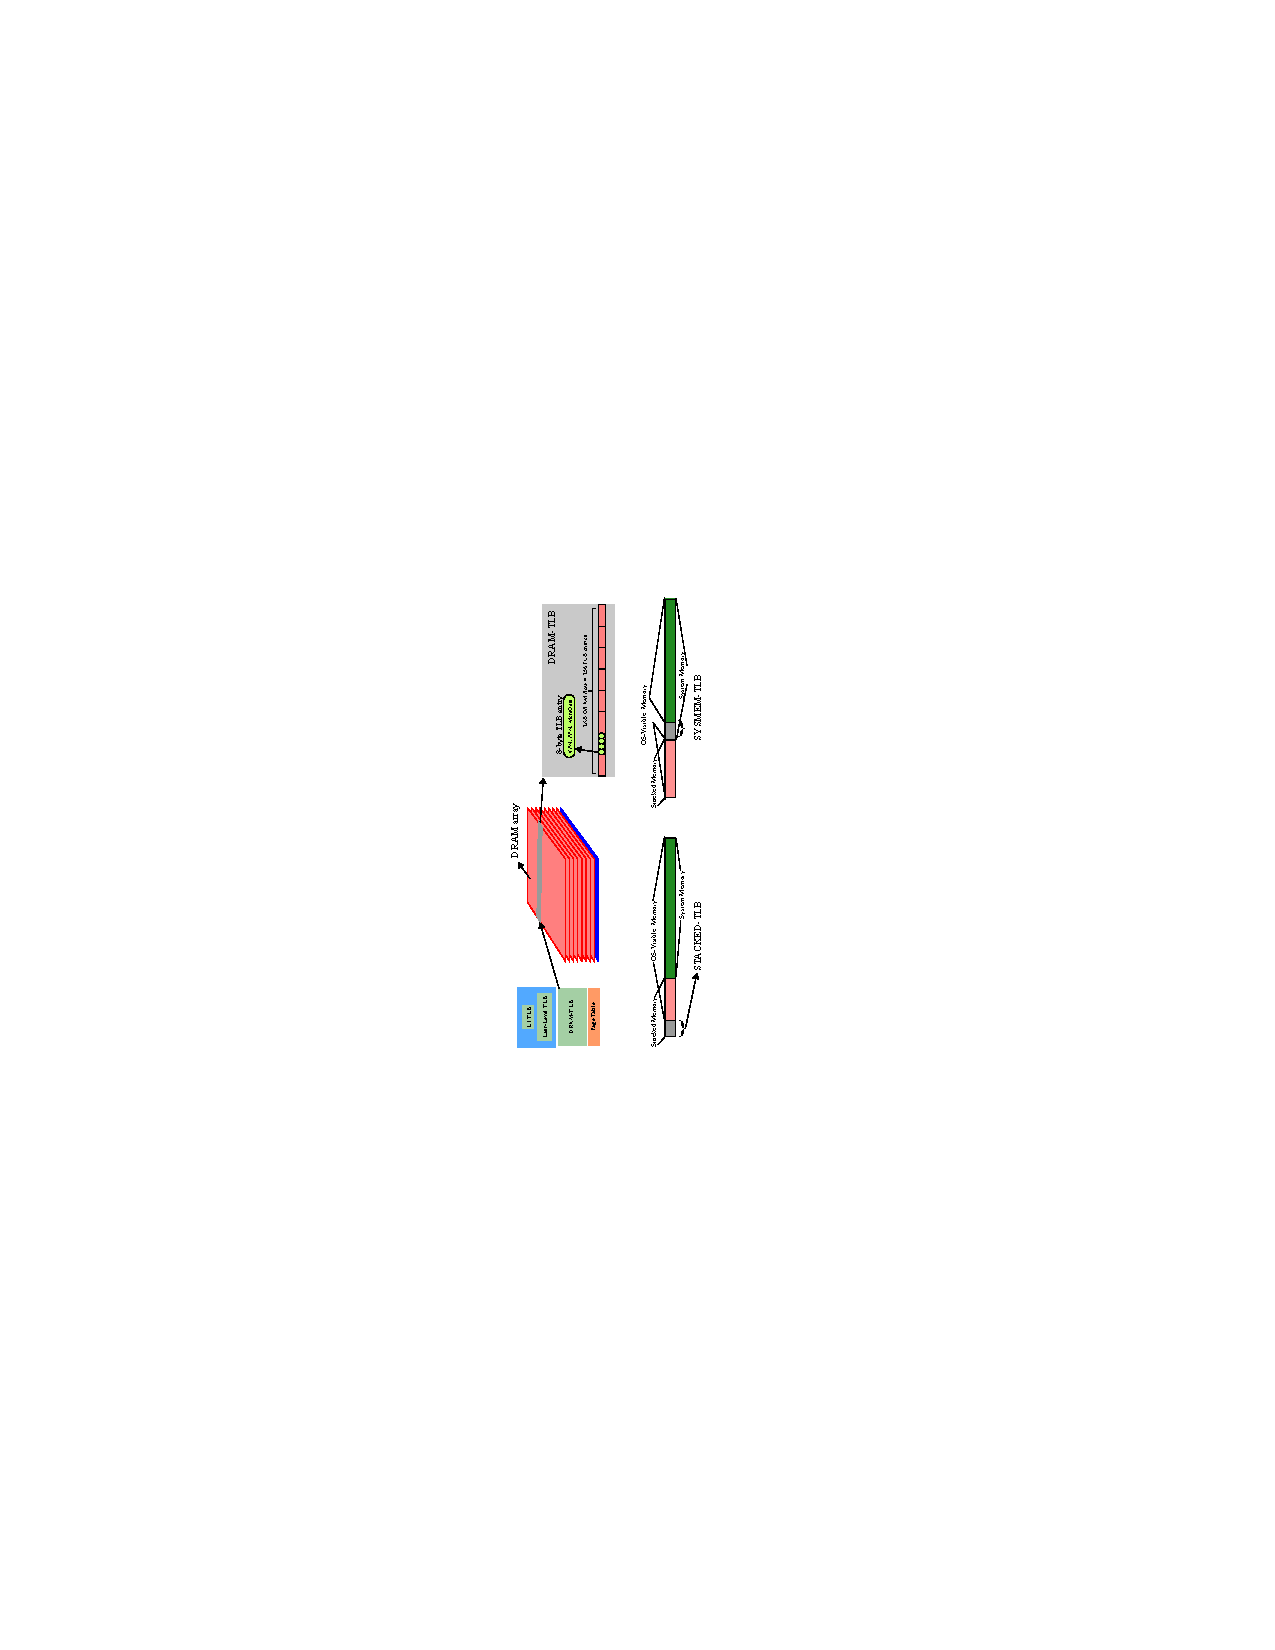
\psfig{file=FIGURES/stacked_tlb,width=\textwidth}}

  \caption{\small Improving TLB coverage by embedding TLBs in DRAM
    (DRAM-TLB). A DRAM-TLB architected using commodity DRAM is called
    SYSMEM-TLB and a DRAM-TLB architected with stacked DRAM is called
    Stacked-TLB. \normalsize}
  \label{fig:stacked_tlb} 
  \vspace{-0. in}
\end{figure*}

\subsection{DRAM-TLB Architecture}

\noindent DRAM-TLBs can either be architected using stacked memory or
system memory. A DRAM-TLB architected using stacked memory is referred
to as a {\em Stacked-TLB} while a DRAM-TLB architected using system
memory is referred to as a {\em SYSMEM-TLB}. DRAM-TLBs are physically
placed in a large contiguous segment of memory and are entirely
hardware-managed. As such, DRAM-TLBs do not contribute to the
OS-visible memory space (see Figure~\ref{fig:stacked_tlb}(c)).

% illustrates, DRAM-TLBs and the OS-visible
% address space when the hybrid memory system is configured with a
% SYSMEM-TLB or a Stacked-TLB.

\subsubsection{DRAM-TLB Organization}

\noindent Like conventional on-chip SRAM TLBs, and the proposed UCAT
architecture, a DRAM-TLB entry maintains the TLB tag, physical
address, and meta data information such as valid bits, page permission
bits, address space identifier (ASID), and the epoch counter (EPCTR).
To accommodate this information, we propose 16 bytes of storage per
DRAM-TLB entry. Figure~\ref{fig:stacked_tlb} illustrates the layout of
the DRAM-TLB in the DRAM array. For example, a 2KB DRAM array holds
128 DRAM-TLB entries per rowbuffer.

\subsubsection{DRAM-TLB Lookups}

\noindent Unlike on-chip TLBs, all DRAM-TLB operations occur on the
DRAM data bus at the granularity of the DRAM read/write interface.
Thus, on an LLT miss, a Stacked-TLB lookup fetches data at the
granularity of the stacked memory interface: 32-byte cacheline (two
TLB entries). While SYSMEM-TLB lookup fetches data at the granularity
of the DDR interface: 64-byte cacheline (four TLB entries).

Reading multiple TLB entries with a single DRAM read operation can be
exploited in two ways. First, retrieving the co-located DRAM-TLB
entries on a DRAM-TLB read naturally enables prefetching of
neighboring address translations. For example, prefetched entries can
potentially be stored in an on-chip TLB prefetch buffer. This approach
is similar to caching co-located page table entries in the page walk
cache on a conventional page table walk. Alternately, reading multiple
TLB entries enables architecting a set-associative DRAM-TLB without
incurring additional latency or bandwidth~\cite{moin2012,loh2011}. 

We explored the design space of set-associative and direct-mapped
DRAM-TLBs. Our studies with both set-associative and direct-mapped
designs yielded similar performance with large DRAM-TLB sizes. These
results match the behavior of existing work on large DRAM Caches where
conflict misses tend to be low~\cite{moin2012}. Thus, we architect a
direct-mapped DRAM-TLB where consecutive DRAM-TLB sets map to the same
rowbuffer in memory (to exploit DRAM row buffer locality). Adjacent
DRAM-TLB entries fetched are also inserted into the PWC for potential
future hits.

% Similar to page walk caches, we also provision an 8-entry
% DRAM-TLB-Cache (DTLBcache) that stores recent lines retrieved from the
% DRAM-TLB. In doing so, the DTLBcache exploits spatial locality in LLT
% misses.

\subsubsection{DRAM-TLB Insertions and Updates}

\noindent The DRAM-TLB must be updated on misses, shootdowns, and page
permission changes. We propose to modify the TLB-entry directly in
DRAM on updates. To ensure that updating a single DRAM-TLB-entry does
not corrupt the contents of co-located DRAM-TLB entries, we leverage
existing DRAM interfaces that allow partial writes (e.g. byte-level
writes) to memory without the power and bandwidth overhead of a full
read-modify-write operation~\cite{hbm-spec}.


% If the DRAM-TLB entry exists in the DTLBcache, the corresponding entry
% is directly updated in the DTLBcache. However, if the entry does not
% exist in the DTLBcache,




% \begin{figure}[htb] 
% \vspace{-0. in}
% \centering
% 	\centerline{\psfig{file=GRAPHS/stackedDRAMTLB_cachelat,angle=-90,width=\columnwidth}}
% 
% \caption{\small This figure compares the average LLC miss latency of
% 	DRAM-TLB and Stacked-TLB relative to the baseline system. \normalsize}
% \label{fig:cachelat_DRAMTLB} 
% \vspace{-0. in}
% \end{figure}

\subsubsection{DRAM-TLB Implementation}

% If the request can be serviced from the first-level page table, the
% MMU follows the baseline address translation policy and fetches the
% translation from the first-level page table. This is because
% retreiving the first-level page table entry and a DRAM-TLB lookup both
% require a single memory access.

% If the MMU is required to access more than one level of the page
% table, we propose that the

\noindent Since the DRAM-TLB is located in physical memory, the
physical location of the DRAM-TLB entry must first be determined. We
propose an 8-byte register in the Memory Management Unit (MMU) to
store the base address $BaseAddr$ for the DRAM-TLB. Given the DRAM-TLB
set index {\em SI} of the missing virtual address, DRAM-TLB
associativity $A$, and DRAM-TLB entry size $s$ (16 bytes in our case),
the DRAM-TLB entry physical address is computed using combinational
logic:

\begin{equation}
  \begin{array}{rl}
    \text{PhysAddr} = BaseAddr + SI * A * s
  \end{array}
\end{equation}

\noindent Once the DRAM-TLB entry is retrieved from memory, a tag
comparison is performed to determine hit or miss. On a DRAM-TLB hit,
the missing translation is returned to the processor. However, on a
DRAM-TLB miss, the application page table is walked to find the
virtual to physical translation. This translation is returned to the
processor and also inserted into the DRAM-TLB for future hits.

\subsubsection{DRAM-TLB Example}

\noindent Assume a 1M-entry direct-mapped DRAM-TLB (with 4KB pages)
starting at memory location {\em BaseAddr=0}. An LLT miss for virtual
page 0xff2212345000 requires fetching the 16-byte DRAM-TLB entry at
set index 0x12345. With $A=1$ and $s=16$, the physical memory location
for this DRAM-TLB entry is 0x123450 (i.e. 0 + 0x12345 * 1 * 16). The
MMU compares the missing tag (0xff22) with the DRAM-TLB entry to
determine DRAM-TLB hit or miss.

\subsection{DRAM-TLB Performance}

% For our evaluation purposes, we do not exploit the prefetching
% benefits from fetching multiple TLB entries with a single DRAM read
% operation.

% \subsubsection{Steady State Performance Behavior}

% Since our application
% have memory footprint less than 32GB, both DRAM-TLB configurations
% incur only compulsory misses and behave like a {\em perfect} DRAM-TLB
% in steady state.

% illustrates the workloads on the x-axis and the performance relative
% to our baseline system on the y-axis. The figure

\noindent We evaluate SYSMEM-TLB and Stacked-TLB performance assuming
an 8-million entry DRAM TLB (32GB TLB coverage with 4KB pages).
Figure~\ref{fig:perf_DRAMTLB} shows that DRAM-TLBs improve performance
relative to the baseline system across all TLB-sensitive workloads. On
average, SYSMEM-TLB improves performance by 11\% while Stacked-TLB
improves performance by 22\%. In general, Stacked-TLBs perform better
than SYSMEM-TLBs because they are architected with stacked memory, a
technology that provides high memory bandwidth and less memory queing
delays. As illusrated in Figure~\ref{fig:tlblat_DRAMTLB}, unlike
SYSMEM-TLBs that reduce address translation latency by 12\% on
average, Stacked-TLBs reduce address translation latency by 40\% on
average. The translation latency reduction stems from the fact that
DRAM-TLBs reduce the number of memory accesses on an LLT miss from 1.6
memory accesses to a single memory access on average (see
Figure~\ref{fig:memaccess_DRAMTLB}). The improved translation latency
boosts performance of workloads like $GUPS$ and $MaxFlow$ by more than
70\%. On the other hand, workloads like $XSBench$, $dmr$, $LULESH$ and
$MiniAMR$ experience more than 15\% performance gain.

% % \subsubsection{Non-Steady State Performance Behavior}
% % 
% % \noindent Under steady state conditions, SYSMEM-TLBs are competitive
% % with Stacked-TLB despite being architected using low bandwidth
% % commodity DRAM. However, in practice workloads tend to go through
% % phases of execution where misses occur in the DRAM-TLB. As such, we
% % now study how SYSMEM-TLBs and Stacked-TLBs behave when they experience
% % TLB misses.
% % 
% % \begin{figure}[t] 
% %   \vspace{-0. in}
% %   \centering
% %   \centerline{\psfig{file=GRAPHS/stackedDRAMTLB_hitrate_sens,angle=-90,width=\columnwidth}}
% % 
% %   \caption{\small Sensitivity to DRAM-TLB hit-rate. \normalsize}
% % 
% %   \label{fig:hitrate_DRAMTLB} 
% %   \vspace{-0. in}
% % \end{figure}
% % 
% % The overhead of a DRAM-TLB miss is the wasted bandwidth to consult the
% % DRAM-TLB and the bandwidth to insert the missing entry into the
% % DRAM-TLB. In general, these operations consume precious DRAM
% % bandwidth. When bandwidth is scarce, both these operations can degrade
% % performance significantly since they do not contribute towards useful
% % work. To understand this phenomenon,
% % Figure~\ref{fig:hitrate_DRAMTLB} illustrates the performance
% % behavior of SYSMEM-TLBs and Stacked-TLBs as a function of
% % hit-rate\footnote{A statistical model that samples a random number
% % generator is used to achieve the desired DRAM-TLB hit rate.}. The
% % x-axis shows the TLB hit rate while the y-axis shows the performance
% % relative to the baseline system averaged across all workloads.
% % 
% % In steady state (i.e. when the TLB hit rate is a 100\%) both
% % Stacked-TLB and SYSMEM-TLB perform well. However, when the hit-rate
% % reduces, DRAM-TLB lookup and DRAM-TLB fill operations start consuming
% % precious DRAM bandwidth. This additional bandwidth quickly degrades
% % SYSMEM-TLB performance. For example, at 80\% hit rate, SYSMEM-TLB
% % performance plunges from 38\% performance improvement to a mere 8\%
% % performance improvement. Continuing to follow the hit-rate curve,
% % SYSMEM-TLBs degrade performance at DRAM-TLB hit-rates below 70\%.
% % These results show that SYSMEM-TLBs are useful only if they can
% % provide near-optimal hit-rate. Unfortunately ensuring a 100\% hit-rate
% % is impossible without future knowledge.
% % 
% % Stacked-TLBs are less sensitive to degradation in hit-rate. An 80\%
% % Stacked-TLB hit-rate retains performance improvement (34\% vs 42\%).
% % Following the hit-rate curve, Stacked-TLBs degrade performance only
% % when the hit-rate drops below 30\% (which is unlikely). Consequently,
% % this suggests that Stacked-TLBs are more suitable alternative to
% % SYSMEM-TLBs. Hereon, we only report performance results for
% % Stacked-TLBs.

% <------------GRAVEYARD
% Both DRAM-TLB and Stacked-TLB improve performance because they reduce
% the address translation bandwidth and address translation latency. In
% doing so, the LLT miss latency reduces by (see ).

% Furthermore, since Stacked-TLBs handle changes in hit-rate gracefully,
% we report performance results for workloads in steady state.

% This suggests that the bandwidth capability of stacked memory enables
% Stacked-TLBs as a viable hardware structure to increase the TLB
% hierarchy.

% Unfortunately, the first order performance bottleneck of DRAM-TLB
% misses is bandwidth. If the DRAM-TLB lookup misses, that is wasted
% bandwidth. Inserting a missing translation into the DRAM-TLB requires
% bandwidth.

% Consequently such requests consume precious system memory bandwidth.
% Furthermore, to DRAM-TLBs

% If DRAM-TLBs can constantly provide hits, they reduce the 1.75 memory
% accesses per LLT miss our workloads observe to a single memory access.
% However, DRAM-TLBs can suffer from misses too. Especially when the
% application footprint exceeds the coverage of the DRAM-TLB. This
% problem can be addressed by simply sizing the DRAM-TLB to cover the
% largest possible application memory footprint. In our experience, the
% majority of DRAM-TLB misses are compulsory misses. Once the workload
% reaches steady state, a DRAM-TLB effectively behaves like a {\em
% perfect} TLB.

% If the workloads frequently miss in the DRAM-TLB, both the latency and
% required bandwidth for address translation increases. This is because
% a DRAM-TLB miss incurs two additional memory accesses: one for missing
% in the DRAM-TLB and the other for inserting the missing DRAM-TLB.


% Note, however that the DRAM-TLB lookup is on the critical path while
% the DRAM-TLB fill can be done in the background. Thus, the memory
% bandwidth penalty of a DRAM-TLB miss is two requests, but the latency
% penalty is one memory access.

% Therefore, the total cost
% of a DRAM-TLB miss is the cost of one memory access serialization latency plus
% any queuing delays due to the DRAM-TLB fill.

% To quantify the desired behavior of DRAM-TLBs, both from miss traffic
% and miss latency perspective, 

% Figure~\ref{fig:hitrate_DRAMTLB} illustrates the required
% DRAM-TLB hit rate to equalize the average address translation traffic
% and the average address translation latency (assuming DRAM-TLB fills
% do not significantly impact memory access latency) respectively. The
% x-axis illustrates the average number of page table memory accesses
% per LLT miss while the y-axis illustrates the required DRAM-TLB hit
% rate.

% Clearly, if the average number of page table accesses per LLT miss is
% one, we would require a 100\% DRAM-TLB hit rate. As described earlier
% in the paper, this would normally occur when the MMU always hits in
% the second-level page table cache. In such situations, the MMU can
% just bypass the DRAM-TLB lookup altogether and just fetch the
% translations directly from the page table.
% 
% However, the majority of our applications require more than one page
% table access per LLT miss (ranging between 1.40 and 2.25). These page
% table access rates require a DRAM-TLB hit-rate ranging between 40\%
% and 80\%. Achieving these hit rates is well within the range of
% DRAM-TLBs because their relative storage overhead is negligible.
% However, in pathological situations where the DRAM-TLB hit-rate is
% well below the desired break-even hit rate (e.g. streaming workload),
% the MMU can dynamically bypass the DRAM-TLB state machine altogether.


% \begin{figure}[t] 
% \vspace{-0. in}
% \centering
% 	\centerline{\psfig{file=GRAPHS/stackedDRAMTLB_break_even,angle=-90,width=\columnwidth}}
% 
% \caption{\small This figure illustrates a sensitivity study for the
%   required DRAM-TLB hit rate for different pagetable requests per LLT miss. \normalsize}
% \label{fig:hitrate_DRAMTLB} 
% \vspace{-0. in}
% \end{figure}
%------------------> GRAVEYARD

\begin{figure}[tp] 
  \vspace{-0.in} \centering
  \centerline{\psfig{file=GRAPHS/DRAMTLB_perf,angle=-90,width=\columnwidth}}

  \caption{\small Performance of DRAM-TLBs. \normalsize}
  \label{fig:perf_DRAMTLB} 
  \vspace{0.2 in}
\end{figure}

\begin{figure}[tp] 
  \vspace{0.in} \centering
  \centerline{\psfig{file=GRAPHS/DRAMTLB_tlblat,angle=-90,width=\columnwidth}}

  \caption{\small Translation Latency Relative to baseline.\normalsize}
  \label{fig:tlblat_DRAMTLB} 
%  \vspace{0.2 in}
\end{figure}

\begin{figure}[tp] 
  \vspace{0.in} \centering
  \centerline{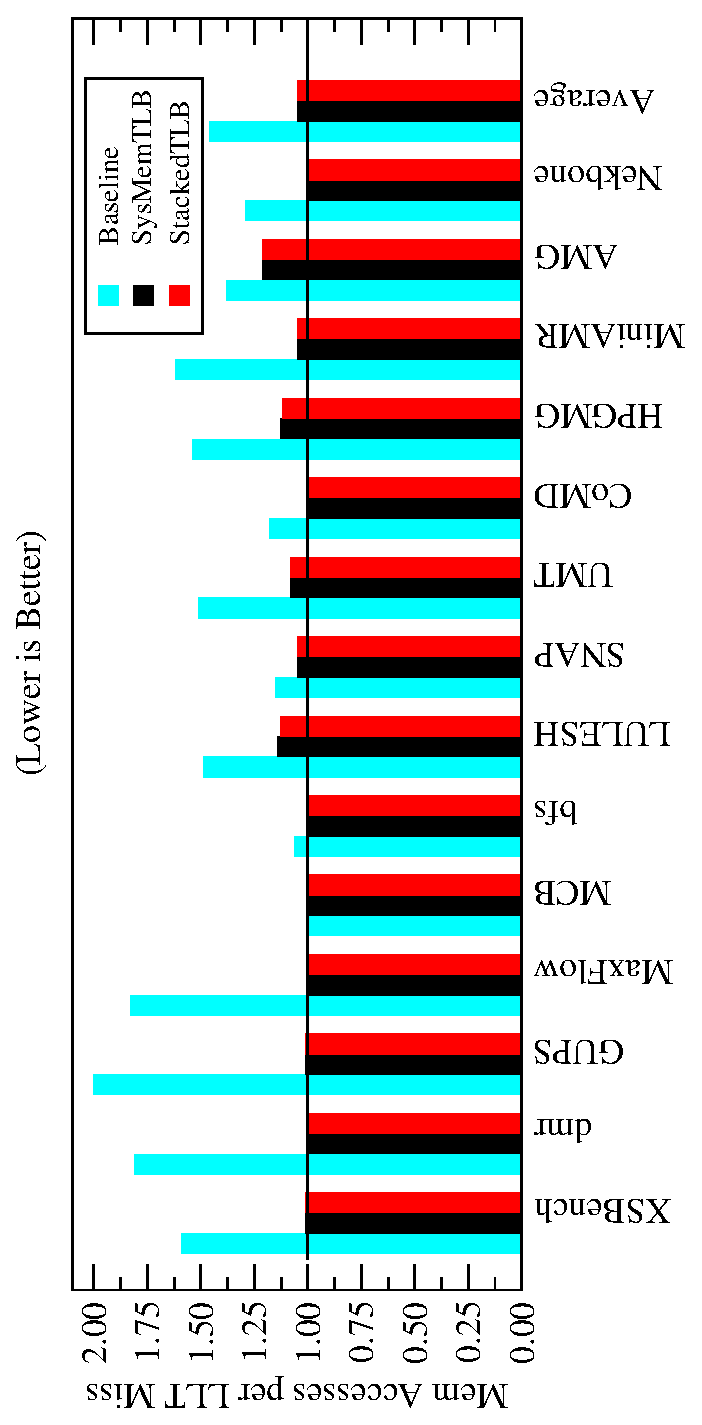
\psfig{file=GRAPHS/DRAMTLB_pteaccess,angle=-90,width=\columnwidth}}

  \caption{\small Memory Accesses on an LLT miss.\normalsize}
 \label{fig:memaccess_DRAMTLB} 
%  \vspace{-0.1 in}
\end{figure}


\subsection{DRAM-TLB Design Overhead}

\noindent We propose simple modifications to the Memory Management
Unit (MMU) state machine to support DRAM-TLBs (see
Figure~\ref{fig:mmu_state}). On an LLT miss, the MMU first consults
the page walk caches to retrieve the translation. If the request
misses in the PWCs, the MMU consults the DRAM-TLB. If the request
misses in the DRAM-TLB, the MMU walks the page table. Thus, we simply
introduce a new state in the MMU state machine for the DRAM-TLB lookup
before walking the page table.

The in-memory storage overhead for DRAM-TLBs depends on the desired
TLB coverage. For example, achieving full system memory (256GB in our
baseline) coverage with 4KB, 64KB, and 2MB pages 1GB, 64MB, and 2MB of
storage overhead (assuming 16-byte DRAM-TLB entries). In general, this
storage overhead is impractical for on-chip SRAM TLBs. However, these
sizes are an insignificant fraction of emerging multi-gigabyte stacked
memory systems. For example, the aforementioned storage overheads
correspond to 6\% (4KB pages), 0.4\% (64KB pages), and 0.01\% (2MB
pages) storage overhead for a 16GB stacked memory system.
Consequently, DRAM-TLBs can improve TLB coverage using small pages
with minimal storage overhead and most importantly require no
significant changes to the existing address translation mechanisms.

\begin{figure}[b] 
  \vspace{-0. in} \centering
  \centerline{\psfig{file=FIGURES/mmu_state,angle=-90,width=\columnwidth}}

  \caption{\small MMU extensions to support DRAM-TLBs.
    \normalsize}
  \label{fig:mmu_state} 
  \vspace{-0 in}
\end{figure}



% \subsection{DRAM-TLB Summary}
% 
% \noindent DRAM-TLB is a flexible, scalable, and low overhead mechanism
% that can provide arbitrary TLB coverage. DRAM-TLB serves as the next
% shared level in the on-chip TLB hierarchy and can reduce memory
% bandwidth requirements for address translation to a single memory
% access and can improve performance by 50\% on average (up to 2X).

% DRAM-TLBs provide an opportunity to increase the coverage of existing
% on-chip TLB hierarchies. Since, DRAM-TLBs can potentially provide
% address translations using in a single memory access, they provide an
% alternative low latency, low bandwidth solution to walking the page
% table on an LLT miss.


